\documentclass[external]{20120615_deliverable_template_ukob}

\usepackage{xspace}
\usepackage{amsmath,amsthm,amssymb,url,color}
\theoremstyle{definition}
\newtheorem{example}{Example}
\usepackage{xcolor}
\usepackage{color, colortbl}
\usepackage{subfigure}
%\usepackage{showkeys}

\newcommand{\todo}[2]{\textcolor{magenta}{#1: #2}}

\LGtitle{\LiveGovThirtyTitleFonts \textbf{D1.2 - Mobile Sensor App with Mining Functionality} }
%\LGnumber{WP.NR} % e.g 6.7 no letters D or ID

\LGnumber{1.2}

\LGwp{WP1 - Reality Sensing and Mining}

\LGdissemination{PU - Public}

\LGcontractdate{Month 27, March 2014}

\LGactualdate{Month 26, February 2014}

\LGtask{T1.1, T1.2, T1.3}

\LGtype{Prototype}

%\LGnature{$<$ Report $|$ Prototype $|$ Demonstrator $|$ Other $>$}

%\LGapproved % activate only if approved
\LGdraft

\LGversion{Alpha 0.4}
%\LGstaffmonths{Resources spent on the deliverable}

%\LGdistribution{WP leaders, PMB members, European Commission}

%\LGkeywords{}


%\LGabstract{Put abstract here (separate paragraphs using
%{\tt\char92 par}.)}
\LGabstract{ 

\todo{HH}{Add abstract}

%  This deliverable describes the mobile sensor mining component.
%  Along with this document we supply the source code of the
%  components, documentation (javadoc), and pre-compiled packages for
%  direct installation and testing on mobile devices.  

}

%\LGhistory{01}{2011-10-01}{First draft}{Yiannis Kompatsiaris}
%\LGhistory{02}{2011-10-02}{Modifications}{Sotiris Diplaris}
%\LGhistory{03}{2011-10-03}{Further Modifications \& Corrections}{Sotiris Diplaris}
%\LGhistory{04}{2011-10-05}{Further Modifications \& Corrections}{Sotiris Diplaris}


%------------------------ macro for change portrait to landscape
\usepackage{calc,graphicx,pdflscape,eso-pic} % needed for printing
                                             % headers and footers
\newlength\landscapewidth
\newlength\landscapeheight
\newcommand\landscapepagestyle{ % command which prepare page
                                % for landscape printing,
                                % change to landscape is
                                % achieved by pdflscape
\clearpage \thispagestyle{empty}
\setlength\landscapewidth{247mm}
\setlength\landscapeheight{161mm}
\AddToShipoutPicture*{\AtPageCenter{ % this make "layer" for
                                     % printing the header and footer
\rotatebox[origin=c]{90}{
\hspace*{-2em} % for adjusting position of
               % header and footer
\parbox{\landscapewidth}{\vskip-.57\landscapeheight
%\centerline{\WEKNOWIT \hfill \textbf{\Large \bf{IDx.x - V0} \normalsize }} %header text for Internal Deliverables
                                                                         % notation: IDx.x V{LGversion}
\centerline{\LiveGovLogo \hfill \textbf{\Large \bf{Dx.x - V0} \normalsize }} %header text for External Deliverables
                                                                        % notation: Dx.x V{LGversion}
\vspace{-5pt} \rule{\landscapewidth}{0.4pt} \\
\rule{0pt}{\landscapeheight} \\
%\rule{\landscapewidth}{0.4pt} \\
\centerline{Page \thepage\ }  % footer text
} } } } }

%--------------------------------------------------------------------------------------------------------------%
\usepackage{appendix}
\pretolerance=10000 % prevent overflow lines for $math$ elements

\begin{document}

% add a \LGaddhistory{version}{date}{reason}{revised by} for each new
% version
\begin{LGhistory}
\LGaddhistory{0.1}{2013-10-14}{Outline}{Heinrich Hartmann}
\LGaddhistory{0.2}{2014-01-06}{Added section on topic modeling}{Christoph Kling}
\LGaddhistory{0.3}{2014-01-07}{Revised Outline}{Heinrich Hartmann}
\LGaddhistory{0.4}{2014-01-07}{Alpha Version}{Heinrich Hartmann}

\end{LGhistory}


\newcommand{\LGaddauthorNoPhone}[3]{\hline  #1 &  #2 & %
   \parbox{3em}{E-mail:} \small #3 \\
}

% add a
% \LGaddauthor{Partner}{Name}{Telephone}{Fax}{Email} for each author
\begin{LGauthors}

\LGaddauthor{UKob}{Heinrich Hartmann}{+49 261 287 2759}%
{+49 261 287 100 2759}{\small hartmann@uni-koblenz.de}

\LGaddauthor{UKob}{Christoph Schaefer}{+49 261 287 2786 }%
{+49 261 287 100 2786}{\small chrisschaefer@uni-koblenz.de}

\LGaddauthor{UKob}{Christoph Kling}{+49 261 287 2702}%
{+49 261 287 100 2702}{\small ckling@uni-koblenz.de}

\LGaddauthorNoPhone{MTS}{Laura Niittyl\"a}%
{\small Laura.Niittyla@mattersoft.fi}

\end{LGauthors}



\begin{LGExecutiveSummary}
  \vspace{10pt} 

\todo{HH}{Add Summary}

\end{LGExecutiveSummary}


% add a \LGaddabbreviation{ABBR}{Explanation} for each abbreviation
\begin{LGAbbreviations}
%\LGaddabbreviation{LG}{Live+Gov}

\LGaddabbreviation{\textbf{API}}
{Application Programming Interface}

\LGaddabbreviation{\textbf{GPS}}
{Global Positioning System}

\LGaddabbreviation{\textbf{GSM}}
{Global System for Mobile Communications}

\LGaddabbreviation{\textbf{HTML}}
{HyperText Markup Language}

\LGaddabbreviation{\textbf{HTTP}}
{Hypertext Transfer Protocol}

\LGaddabbreviation{\textbf{JSON}}
{JavaScript Object Notation}

\LGaddabbreviation{\textbf{REST}}
{Representational State Transfer}

\LGaddabbreviation{\textbf{SVM}}
{Support Vector Machine}

\LGaddabbreviation{\textbf{URL}}
{Uniform Resource Locator}

\LGaddabbreviation{\textbf{UUID}}
{Universal Unique Device Identifier}

\LGaddabbreviation{\textbf{WP}}
{Work Package}

\LGaddabbreviation{\textbf{WIFI}}
{Wireless Fidelity (IEEE 802.11), WLAN}

\LGaddabbreviation{\textbf{WLAN}}
{Wireless Local Area Network}

\LGaddabbreviation{\textbf{XML}}
{Extensible Markup Language}

\LGaddabbreviation{~\\}
{~~~}

\end{LGAbbreviations}

% add a \LGaddterm{Term}{Explanation} for each entry of the glossary
%\begin{LGGlossary}
%\LGaddterm{Term}{Definition text here}
%\LGaddterm{Term2}{Definition text here}
%\end{LGGlossary}

\setcounter{tocdepth}{1}

% add this for a table of contents
\LGTOC

\newpage

\chapter{Introduction}
\label{chap:Introduction}
\todo{HH}{Write Introduction}

\section{Description of Deliverable D1.2}
Sensor Data App with Mining Functionality: This deliverable will provide the
extended version of the data capturing prototype for mobile devices, with
implemented reality mining methods and optimized communication interfaces for
result transmissions for to the application server.

\section{Task Descriptions}
\begin{itemize}
\item[T1.1] {\bf Sensor and user input data capturing} \\
  This task will first define a taxonomy of classifications that are useful to
  determine for contextualization of citizens’ uploads including activity
  profiles (e.g. walking, cycling, riding train, riding bus,...) and coarse
  issue classifications (street, people, traffic,...). Research investigations
  will determine how these categories can be captured and classified
  economically using limited battery power (e.g. trading off between power
  draining sensors like GPS or audio by less expensive ones like accelerator
  monitoring) and limited bandwidth to the Live+Gov backbone server. The task
  also comprises the contextualized capturing of citizen text, deictic or voice
  input while accounting for limitations of mobile hardware and communication
  channels.
\item[T1.2] {\bf Smartphone based reality mining} \\
  In this task we will develop memory and energy aware mining mechanisms for
  exploiting data collected in T1.1 for various kinds of initial processing on
  mobile devices - including classification, filtering, abstraction, and
  personalization. The key concern of our development will be on wide usability
  of reality mining methods and their flexible applicability for dynamic user
  contextualization in project scenarios.
\item[T1.3] {\bf Server based reality mining} \\
  Based on limited analysis of data in T1.2 and based on citizens’ preferences
  and explicit consent, (possibly) abstracted sensor data will be uploaded to
  the Live+Gov backbone where further mining will occur. We will develop mining
  methods which are needed for the application, but cannot be run on individual
  smartphones (e.g.  because input from multiple users is needed). In
  particular, this will comprise the detection of common patterns delivered from
  many citizens, but also outlier detection and treatment, which is required to
  discover spoofing or important emergencies. The methods resulting from this
  task will be particularly relevant for supporting augmented reality
  applications (WP3) and contextualization of data mining results in eGovernance
  scenarios in line with policy models (WP2).
\end{itemize}


\clearpage
\chapter{Sensor Collection Service}
\todo{HH}{Add content}

Explain the improvements of the sensor collection service since D1.1

In particular cover the topics:
\begin{enumerate}
\item Improved Architecture Description
\item Inspection Front End
\item New Sensor Transfer File Format
\item New Streaming API
\item Integration Loging and Heartbeating into Upload Servlet
\item Data Collection event in Koblenz
\end{enumerate}

\chapter{Reality Mining Methods}

\section{Human Activity Recognition}
\todo{HH}{Add content.}

\subsection{Related Work}
Explain common approaches to human activity recognition, evaluation
methods and resulted quality.

\subsection{Component Description}
Explain our own implementation:

\begin{enumerate}
\item Architecture Description (Class diagrams, DB Schemes)
\item Decision Tree classifier
\item PCA-SVM based classifier
\end{enumerate}

\subsection{Cross-Platform Strategy}
Explain problems with Titanium framework.

Android component runs on Blackberry. 

Implement HAR as SAAS. Write client app for iOS.

\subsection{Evaluation}
Comparison of our classifier with literature on the basis of external
data sets.

\section{Service Line Detection}

One part of the user contextualization is the service line detection. The aim of this component is to recognize if a citizen uses public transport within the HSL area in Helsinki. If such a usage is detected, the right service line id with its direction and the further itinerary will be determined. Based on this information it is possible to solve higher level tasks like traffic jam detection, connecting train recommendation, or network utilization analysis.

The service line detection is implemented as a server side mining component which provides a REST API for answering user queries in real time. For long term evaluations all API calls are recorded and send to the L+G Service Center on a daily bases. Due to the seamless integration into the L+G ecosystem, where each user gets an universal unique id, all received tracks are personalized and can be combined with additional information coming from other components. In a later analysis, the service line detection results can be augmented with the low level human activity recognition data of the same user to gain a better insight into the users behavior.

\begin{figure}[ht]
\centering
\subfigure[]{
  \frame{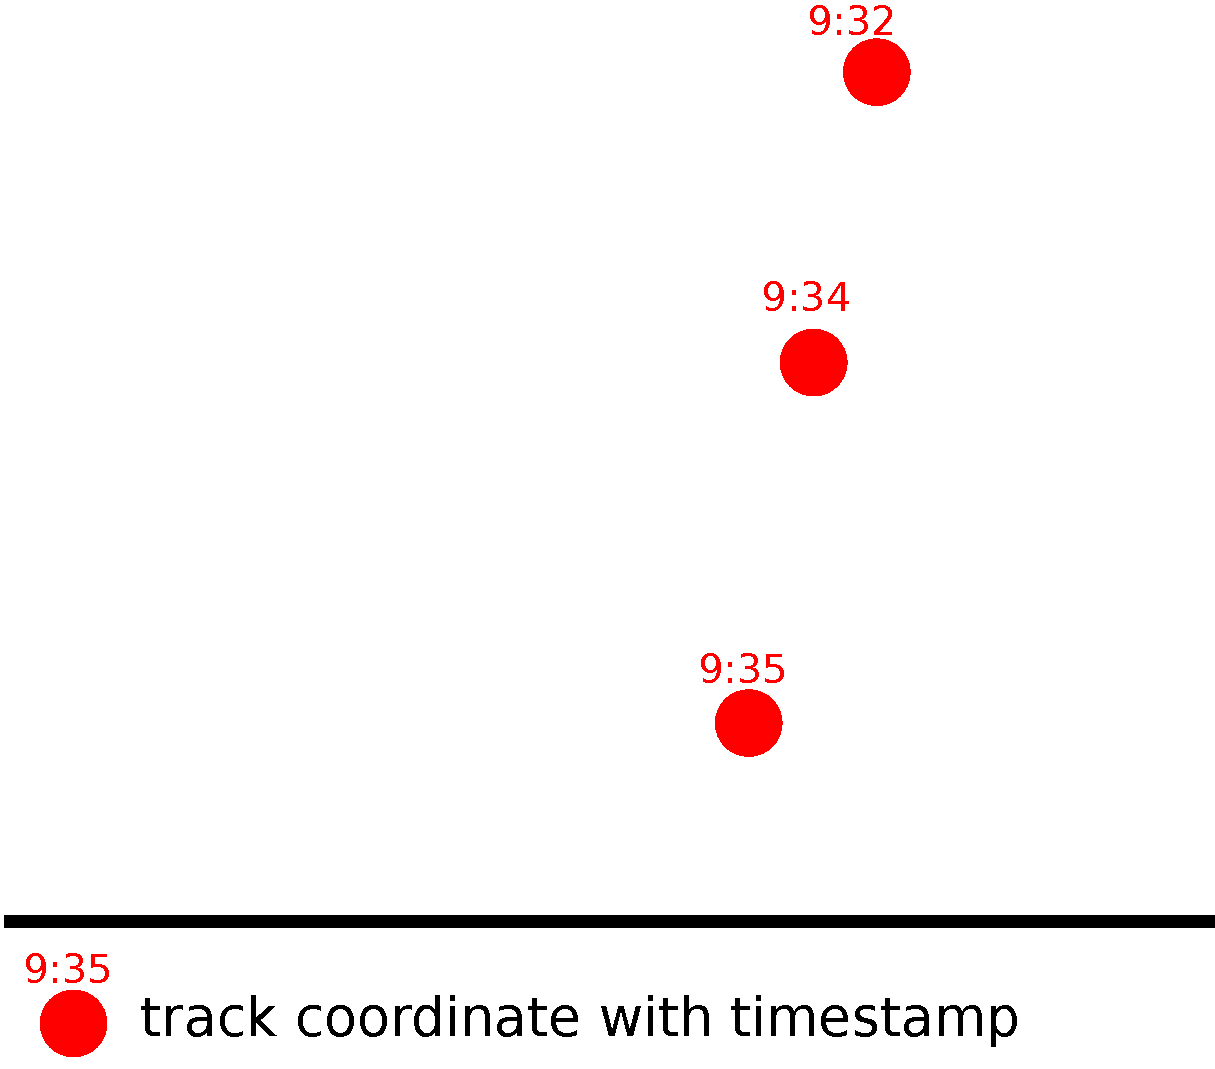
\includegraphics[width=0.3\textwidth,natwidth=556.19,natheight=432]{img/SLD/track.pdf}}
  \label{fig:track}
  \setcounter{subfigure}{1}
} 
\subfigure[]{
  \frame{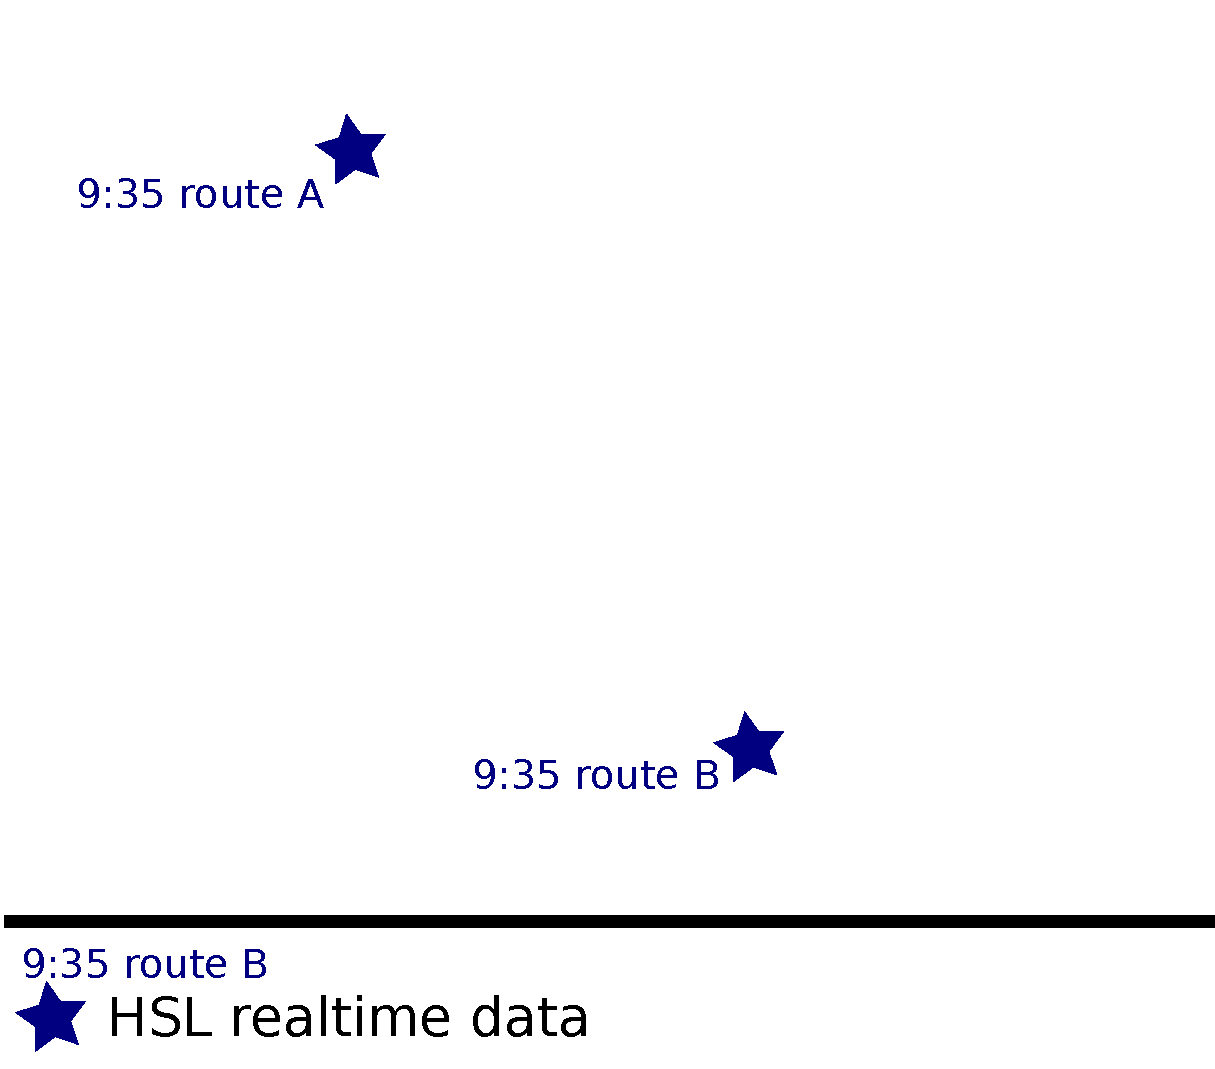
\includegraphics[width=0.3\textwidth,natwidth=556.19,natheight=432]{img/SLD/realtime.pdf}}
  \label{fig:realtime}
  \setcounter{subfigure}{2}
}
\subfigure[]{
  \frame{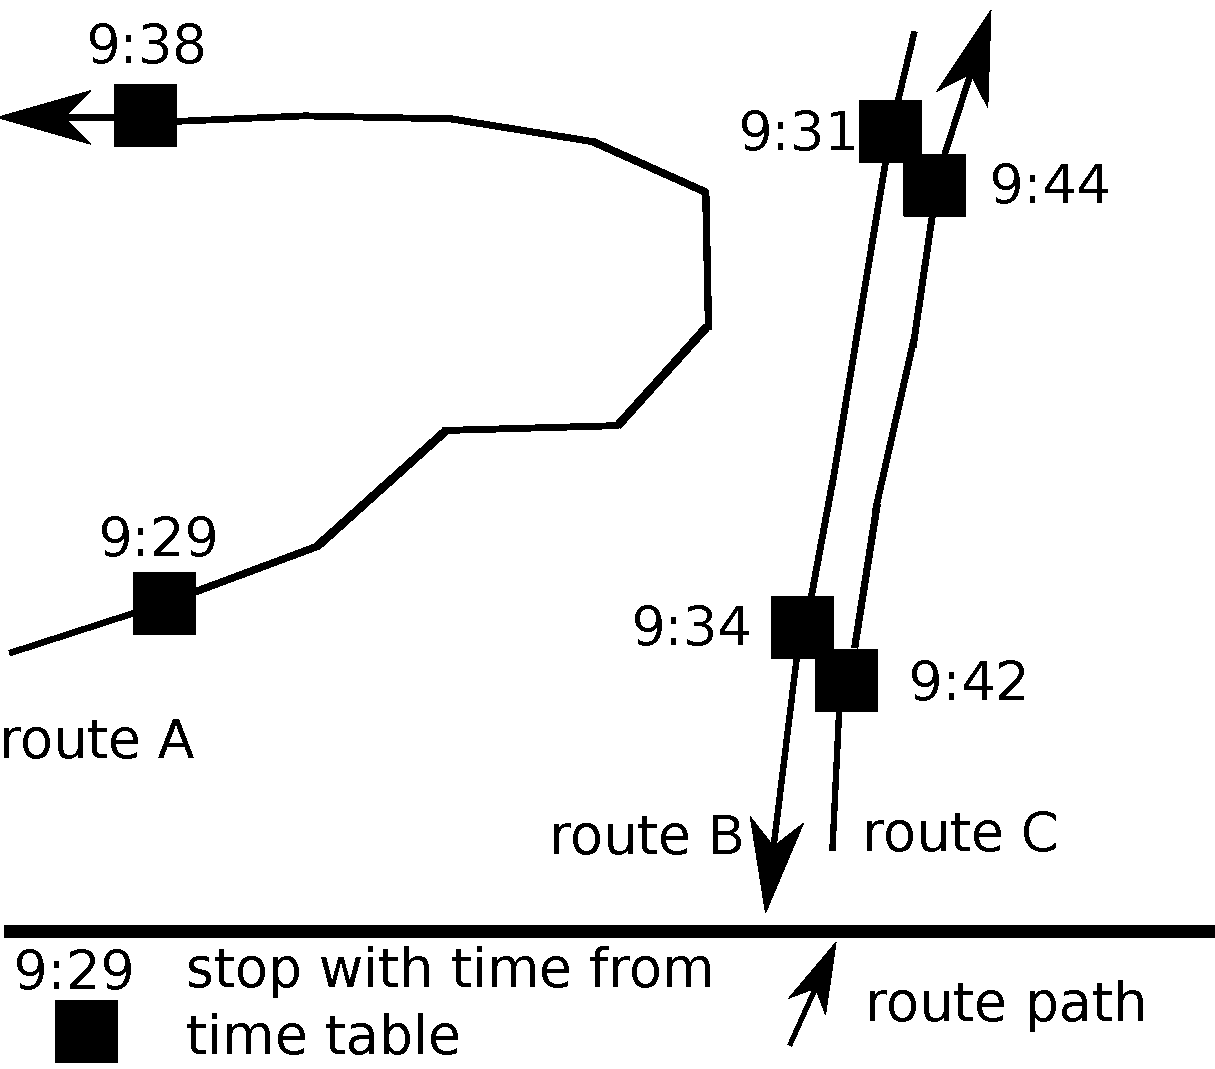
\includegraphics[width=0.3\textwidth,natwidth=556.19,natheight=432]{img/SLD/static.pdf}}
  \label{fig:static}
  \setcounter{subfigure}{3}
}
\subfigure[]{
  \frame{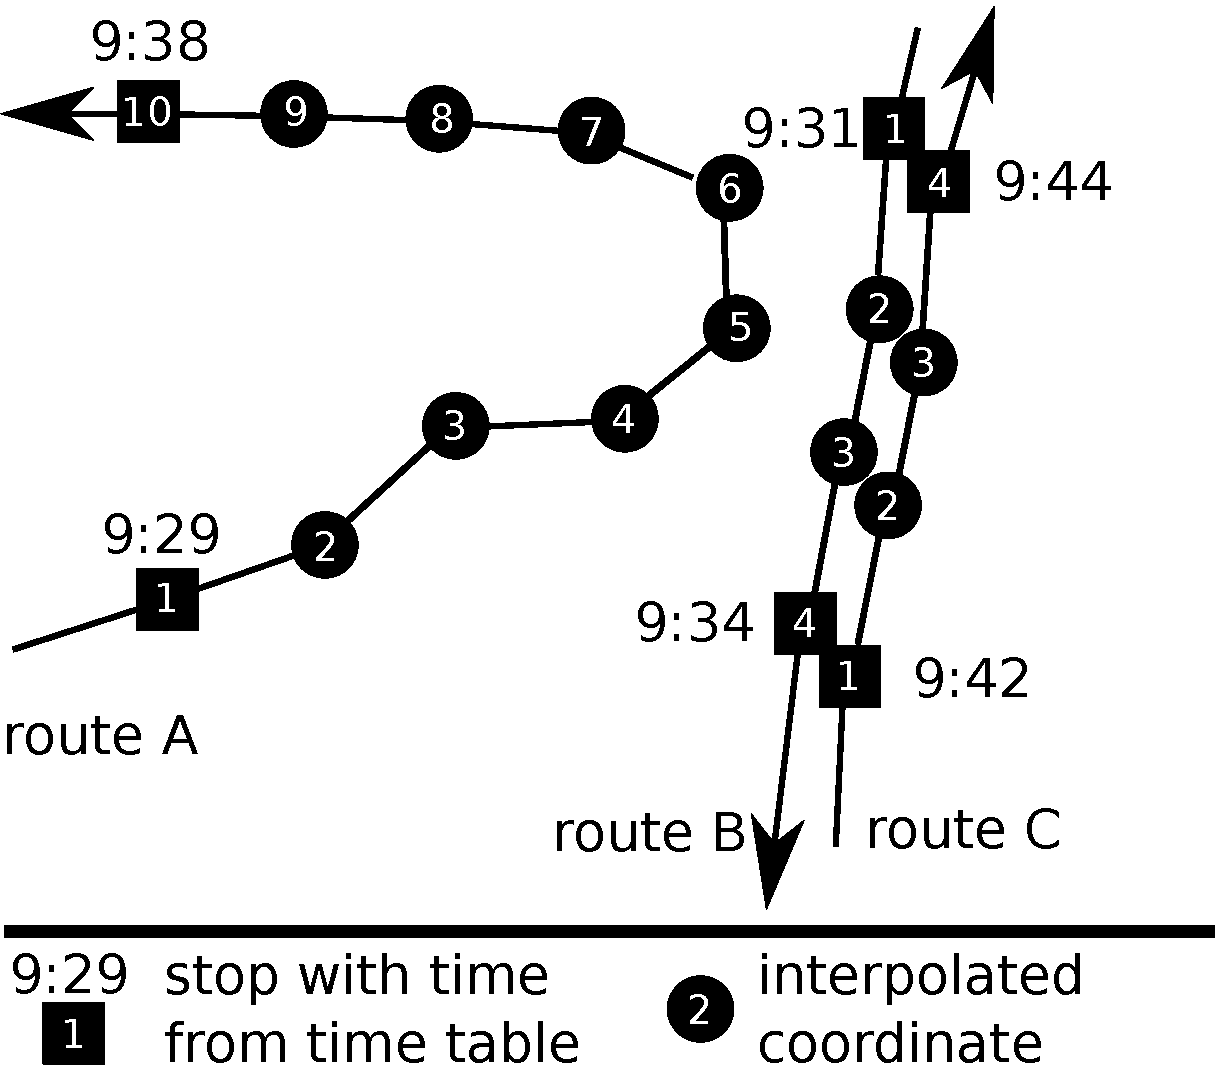
\includegraphics[width=0.3\textwidth,natwidth=556.19,natheight=432]{img/SLD/interpolatedCoords.pdf}}
  \label{fig:interpolatedCoords}
  \setcounter{subfigure}{4}
}
\subfigure[]{
  \frame{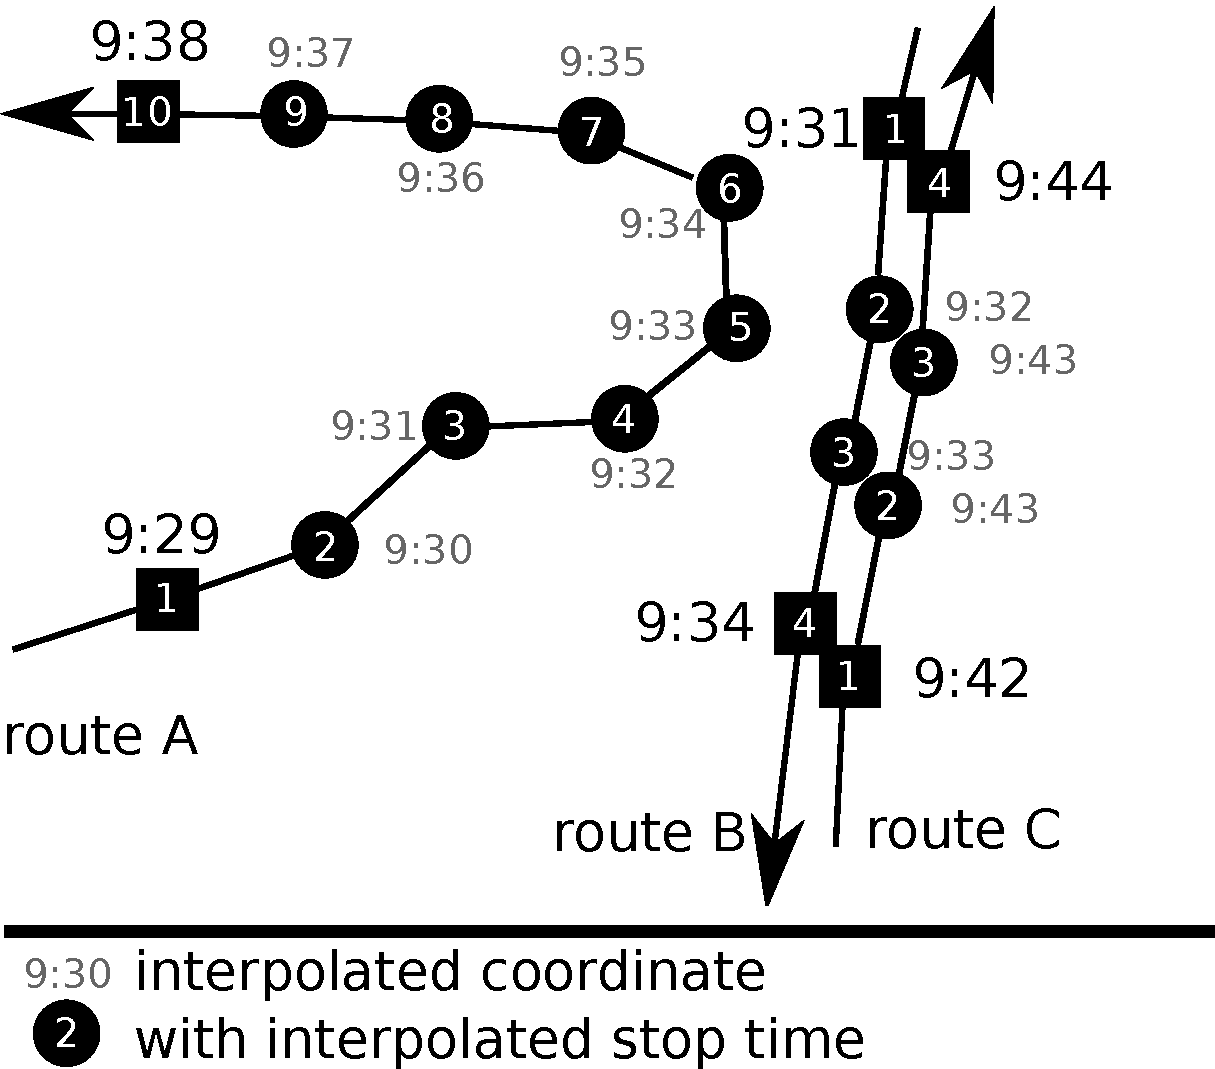
\includegraphics[width=0.3\textwidth,natwidth=556.19,natheight=432]{img/SLD/interpolatedCoordsWithTimes.pdf}}
  \label{fig:interpolatedCoordsWithTimes}
  \setcounter{subfigure}{5}
} 
\subfigure[]{
  \frame{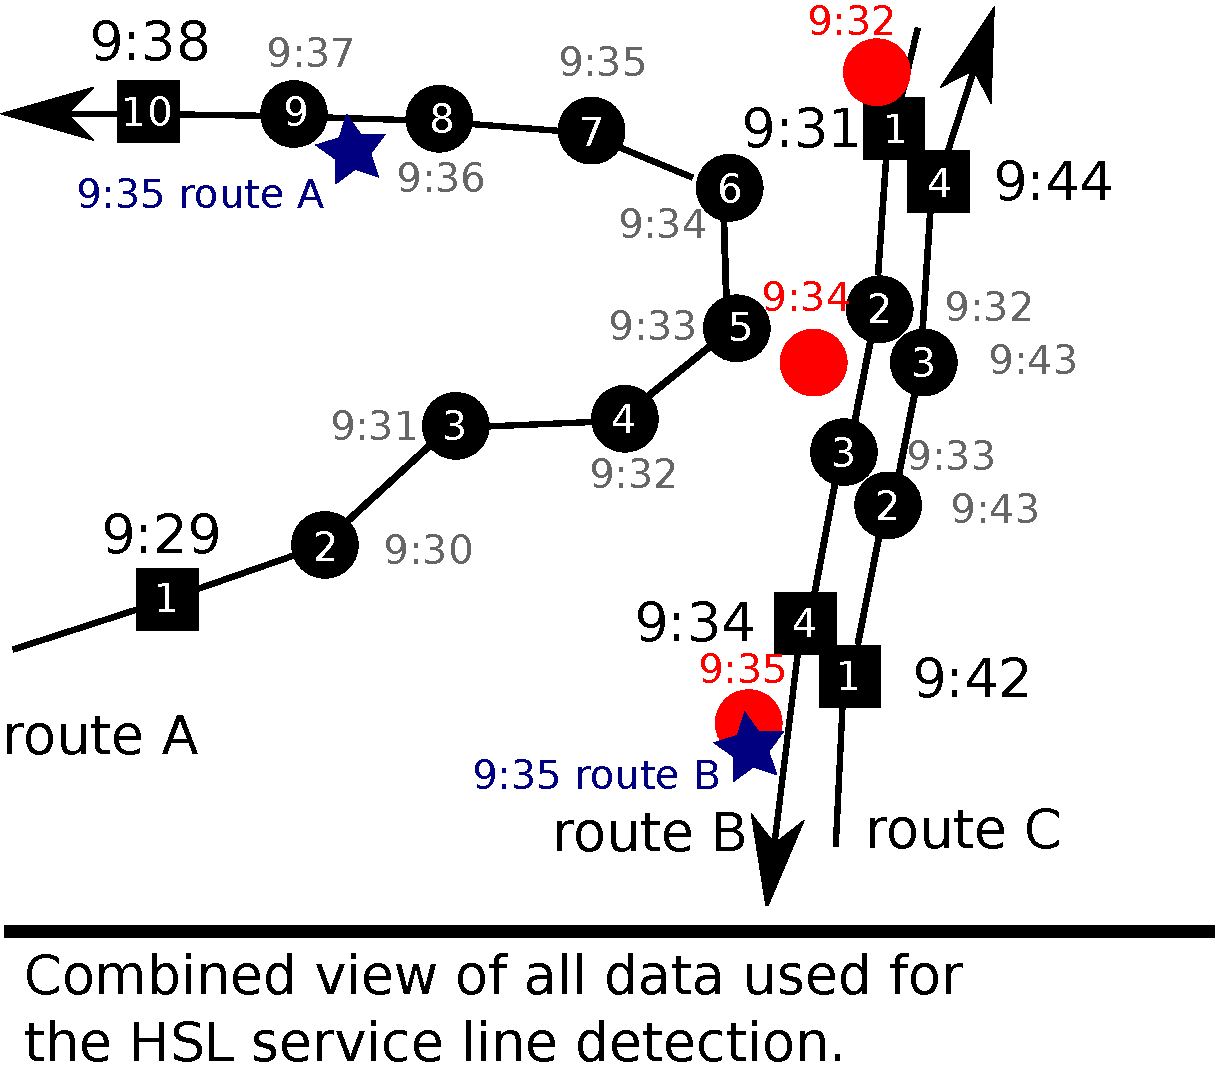
\includegraphics[width=0.3\textwidth,natwidth=556.19,natheight=432]{img/SLD/combined.pdf}}
  \label{fig:combined}
  \setcounter{subfigure}{6}
}
\caption{
The various input data for the HSL service line detection.
}
\label{fig:SLD}
\end{figure}

Assigning a trajectory to a specific service line requires the access to suitable background knowledge. In the Helsinki case it is two fold:
First of all, the system is fed with all HSL public transportation schedules and associated geographic information. By means of this dataset the theoretical position of every vehicle at any point in time can be calculated. A drawback of only including static time tables is that actual schedule deviations stay disregarded. This gap is closed by the HSL Live API, which is the second data source the service line detection relies on. With this API, the actual positions of some vehicles can be determined. Especially trams are tracked in realtime and can be accessed via this interface.  Unfortunately, the vast majority of vehicles, such as buses, have not yet been integrated. Lacking a complete realtime coverage is why still some uncertainty remains in the overall system. Therefore, the main challenge is to combine both kinds of data to archive the best possible performance.

Just as the background data, the classification algorithm is also two-stage. Given a user trajectory containing a small set of GPS coordinates with timestamps (Figure~\ref{fig:track}), in a first step is checked if the most actual given timestamp is near the actual time. If so, the HSL Live API is called in order to find all vehicles which are currently around the user (Figure~\ref{fig:realtime}). Service lines found below a certain distance to the user are scored with a high probability to be the true line belonging to the given track.

In a second step, each coordinate of the given track is compared to the static route data (Figure~\ref{fig:static}) obtained from the time tables. 
It should be noted that the public transportation schedules only contain exact arrival times for each stop, but don't provide any time data for the pathes between them. Since this data is too sparse to perform reliable service line detection on it, all paths are rasterized evenly (Figure~\ref{fig:interpolatedCoords}) and the corresponding time for each intermediate part is interpolated (Figure~\ref{fig:interpolatedCoordsWithTimes}). This ensures that no route section falls through the cracks when executing a simple distance query in time and space. Figure~\ref{fig:combined} shows the combined view of all data used for the HSL service line detection.

The result of the algorithm is the one service line which has the highest score due to the Live API and/or the smallest distance to the given set of coordinates. During a testing phase, the optimal values of all involved parameters like distance thresholds, time and space raster sizes, and the individual scoring weights have to be learned. As one outcome of the Helsinki field trial, we expect to find a good heuristic how to setup the various ingredients of the algorithm.

\subsection{Implementation details}
As a starting point, HSL provided us with all static service line data like arrival times, stop positions, route meta data, and shape files in the well known General Transit Feed Specification (GTFS)\footnote{\url{https://developers.google.com/transit/gtfs/}}. The origin data set had a size of 400 MB and was imported into a PostgreSQL database. All shapes and stop positions were stored as native geospatial values using PostGIS, a spatial database extender for PostgreSQL. After the import, we found 587 distinct routes, 7534 stops, and a total number of 206,153 trips in the database. In general, a route like the bus 934 from Myyrm\"{a}ki to Luhtaanm\"{a}ki, has two directions, travels along its route shape and stops at its stops. If a service line runs every ten minutes, each trip has its own trip id and is uniquely identifiable.

While these data are too sparse for distance queries, we interpolate every trip to ensure that the distance between two consecutive trip positions is always smaller than ten meter. On the one hand, this simplifies a query like "find all trips in a distance of 20 meters around the user which arrive in plus minus one minute from now" a lot. On the other hand, the interpolation and denormalization inflates the data. Resulting in 324,440,457 trip positions annotated with arrival time and trip id, we enlarged the original data to a size of 38 GB.

This size leads the PostGIS index to its limit and prevents response times below 30 seconds for a service line detection query. Therefore, all data was partitionated horizontally in time dimension. The reason is, that all time tables repeat itself every 7 days and an usual query covers only a very small period of time at a specific weekday. Against this background, we divided the data into 24 parts for every day, which results in 7 times 24 subtables in the database. Finally, this setting archives average response times of less than one second for a whole service line detection query, containing of up to 200 single distance queries.


\subsection{Evaluation}
How did we test the quality of the classifier.

\section{Traffic Jam Detection}
\todo{MTS}{Add content.}

\subsection{Related Work}
Explain common approaches to Traffic Jam detection or related problems.

\subsection{Component Description}
Explain implementation. 

\subsection{Evaluation}
How was the quality of the jam detection classifier assessed?

\section{Distributed Geo-Matching}
\todo{DJ}{Add content.}
%--------------------------------------------------------------------
%\chapter{Example Section}
%--------------------------------------------------------------------

%%% Local Variables: 
%%% mode: latex
%%% TeX-master: "../D1-2"
%%% End: 

%\subsection*{Geographical Data and Social Media}

Nowadays, the means of public transportation become equipped with physical sensors like GPS sensors or light barriers. Those sensors are used to keep track of the current vehicle position or to estimate the number of passengers. But those sensors do not detect, for instance, emergencies, accidents or the passengers' opinions on bus lines. To overcame these limitations, another kind of sensors is required.

In the last decade, many social networks or micro-blogging services like Twitter\texttrademark arose. They are frequently used by humans to publish their opinions, observations, etc. which then can be requested by a web API. Therefore, the users of those services can be seen as social sensors. The increasing number of mobile phones leads to a situation in which more and more passengers become social sensors by publishing statements about crowded buses or rioting passengers.

The evaluation of the social sensor data requires that the bus or train can be identified to which a message is related. This task is simplified by the fact that most mobile phones have integrated GPS sensors. They measure the current geographical position, which is added to the published message together with a timestamp. This position information can be used to identify the nearest train or bus. A more detailed description of this matching problem  will be given in the next section.

The amount of data produced by the different types of sensors can exceed the processing capabilities of a single computer. Therefore, a distributed approach is required, which will be explained in section \ref{sec:approach}. Finally, the results of an experiment with the current implementation are presented in section \ref{sec:experiment}.

\subsection{Problem of Matching Physical and Social Sensor Data}\label{sec:problem}

In order to find the bus or train a message is related to, the data measured by the physical sensors have to be processed first. In this context, the relevant data consists of the longitude and latitude measured by the GPS sensors of the vehicles. Before transmitting these data, they have to be extended by the unique id of the current vehicle and a timestamp to keep track of the chronological order. The set of all possible position is defined as $Pos$ in equation (\ref{eqn:Pos}).

\vspace*{-2\baselineskip}
\begin{eqnarray}
 Pos & := & V_{id} \times T \times \mathbb{R} \times \mathbb{R}\label{eqn:Pos}
\end{eqnarray}

The relevant data of the social sensors are the messages published by the passengers. Each message contains a timestamp, i.e., the publishing time and the GPS position of the mobile phone from which the message was sent. The set of all possible messages $Mes$ is defined in equation (\ref{eqn:Mes}) where $C$ is the set of all possible message contents.

\vspace*{-2\baselineskip}
\begin{eqnarray}
 Mes & := & T \times \mathbb{R} \times \mathbb{R} \times C\label{eqn:Mes}
\end{eqnarray}

The data of the different sensors are transmitted as a not necessarily finite stream of data as defined in the equations (\ref{eqn:posStream}) and (\ref{eqn:mesStream}).

\vspace*{-2\baselineskip}
\begin{eqnarray}
 posStream: &  & \mathbb{N} \rightarrow Pos\label{eqn:posStream}\\
 mesStream: &  & \mathbb{N} \rightarrow Mes\label{eqn:mesStream}
\end{eqnarray}

The range of $posStream$, i.e., the set of vehicle position received by the data stream $posStream$ are the trajectories of the different vehicles. A trajectory is defined in equation (\ref{eqn:traj}) as a discrete function mapping some point in time to a geographical position.

\vspace*{-2\baselineskip}
\begin{eqnarray}
 traj: & & T \mapsto \mathbb{R} \times \mathbb{R}\label{eqn:traj}
\end{eqnarray}

But this definition is not adequate because the timestamps of messages may vary from the timestamps contained in the position data of the vehicles. Therefore, a continuous trajectory function $\widehat{tray}$ is required. This is reached by, for instance, a linear interpolation of $tray$.

Equation (\ref{eqn:allTraj}) shows the function $allTraj$ which maps the unique identifier of a vehicle on its corresponding continuous trajectory.

\vspace*{-2\baselineskip}
\begin{eqnarray}
 allTraj: & & V_{id} \mapsto (T \mapsto \mathbb{R} \times \mathbb{R})\label{eqn:allTraj}
\end{eqnarray}

In order to relate a message $m$ to a bus or train, the vehicle must be determined which has the smallest euclidean distance $dist$ to the position of the sender at the point in time when $m$ was sent. Furthermore, a vehicle has a maximum length $maxDist$ and all vehicles with a greater distance from $m$ can be ignored. Thus, each message can be seen as a range nearest-neighbour query $rnn$ as defined in equation (\ref{eqn:rnn}).

\vspace*{-2\baselineskip}
\begin{eqnarray}
 &&rnn: Mes \rightarrow Pos \cup \{\texttt{null}\} \textrm{ with}\label{eqn:rnn}\\
 &&rnn((t,lon_m,lat_m,cont)):= (vId,t,lon_v,lat_v)\nonumber\\
 &&\hspace*{1cm}\textrm{if } allTraj(vId)(t)=(lon_v,lat_v) \wedge dist((lon_m,lat_m),(lon_v,lat_v))\leq maxDist \wedge \nonumber\\
 &&\hspace*{1cm}\not\exists vId' \in V_{id}: dist((lon_m,lat_m),allTraj(vId')(t))< dist((lon_m,lat_m),allTraj(vId)(t))\nonumber\\
 &&rnn((t,lon_m,lat_m,cont)):= \texttt{null}\nonumber\\
 &&\hspace*{1cm}\textrm{otherwise}\nonumber
\end{eqnarray}

Putting it all together, the problem of finding the nearest vehicle for each message is defined as followed:

{
\definecolor{mygray}{gray}{.75}
\fbox{\colorbox{mygray}{\parbox{\columnwidth}{
\textbf{Problem} Finding range nearest vehicle for each message\\
\textbf{Input:} $posStream$, $mesStream$, $maxDist$\\
\textbf{Output:} $rnnStream: \mathbb{N} \rightarrow Mes \times Pos \bullet rnnStream(i):=(mesStream(i),rnn(mesStream(i)))$
}}}
}

An implementation which solves this problem has to deal with the fact, that the data received by different sensors are not equally delayed. For instance, the data measured from physical sensors may be faster transmitted then messages received from social networks.

Another difficulty is, that the amount of data received by the different input streams may exceed the processing capabilities of a single computer. One solution for this problem would be to discard incoming data if the load of the single machine would be to high. This could lead to the loss of valuable data. In order to avoid this, a distributed approach is required which scales horizontally.

Some approaches like PLACE* \cite{Xiong2007PAD} distribute the incoming data according to a static mapping of computers on geographical regions. The disadvantage of this static mapping can be seen, for instance, if there exists a sport stadium in some region. If a sport event takes place, then there are many vehicles and passengers producing a huge amount of data. Therefore, the corresponding computer can only deal with a relatively small region. But if not event takes places, this computer does nearly have no work. In order to improve this, the mapping has to be dynamic, i.e., a dynamic load balancing is required.

\subsection{Distributed Geo-Matching Approach}\label{sec:approach}

The schema of an intuitive stream-processing system which solves the problem described above can be seen in figure \ref{subfig:localRtree}. It consists of a single component ($C$) which receives the incoming data streams of vehicle positions and messages. It caches the current positions and processes the range nearest-neighbour queries initiated by the received messages. The answers are transmitted via the outgoing data stream $rnnStream$.

In order to answer range nearest-neighbour queries, $C$ has to cache the current position of all vehicles. The problem of the delayed sensor data requires the caching of more vehicle positions than just the latest. Thus, a sliding window approach is implemented with a window size exceeding all regular delay times. This is realized by deleting all vehicle positions outside the window whenever a new position with a timestamp later then the timestamp of the latest cached position is received.

The data structure used as cache should answer range nearest-neighbour queries efficiently. In spatio-temporal databases R*-trees \cite{Beckmann1990TRA} are used for this purpose. Similar to a B-tree, the inserted elements are stored only in the leafs. Each node except the root has a minimal and a maximal number of children or elements. If an insertion is performed on a node already containing the maximal number of elements, then it is split and the resulting inner node is inserted in the parent node. In contrast to B-trees, each node of an R*-tree represents the minimal bounding rectangle (MBR) of all elements contained in its subtree as illustrated in figure \ref{fig:Rtree}. The presented tree consists of a root node (dark gray), seven leafs (light gray) and several vehicle positions (black squares).

\begin{figure}[htbp]
\centering
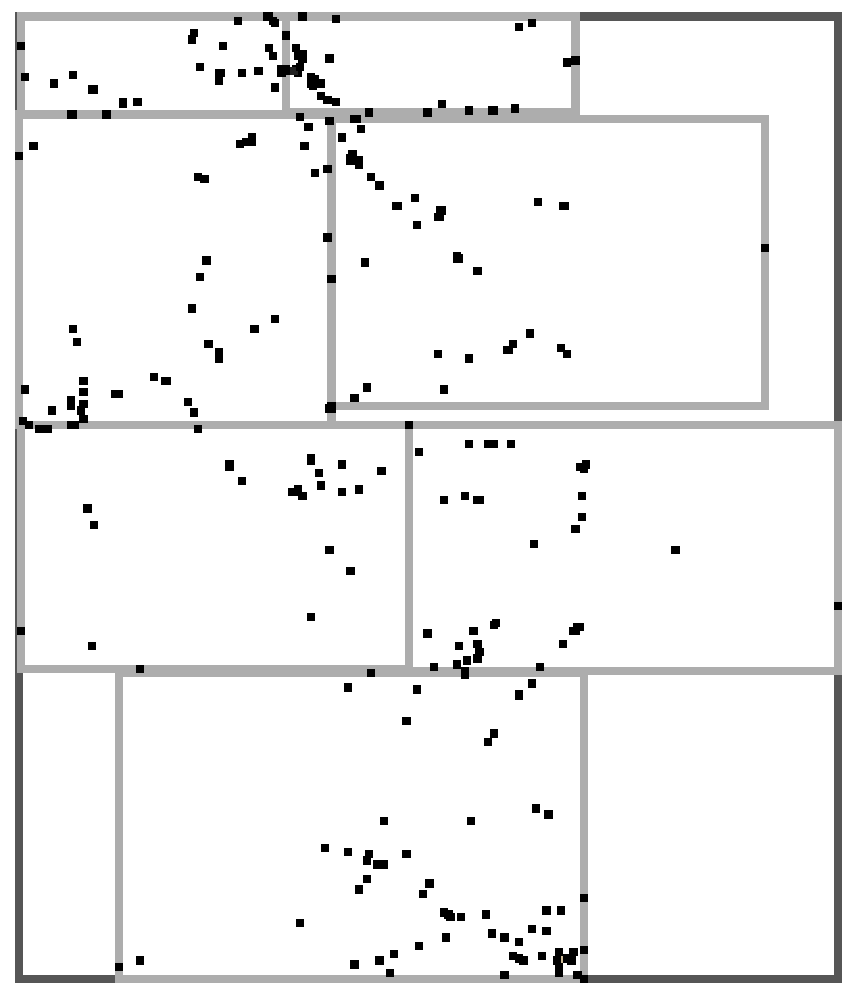
\includegraphics[scale=0.3,angle=90]{img/dgm/rTree.pdf}
\caption{An examplary R*-tree}\label{fig:Rtree}
\end{figure}

During the processing of a range nearest-neighbour query, only the children of a node are visited whose MBR intersects with the queried range. Thus, the performance of the query processing depends on the number of subtrees to be traversed. In order to reduce this number, the MBRs of the child nodes should be disjoint. As shown in \cite{Beckmann1990TRA} the algorithms used for insertion and deletion are designed to ensure a minimal overlap of MBRs. Another advantage is, that the MBRs are dynamically adjusted according to the currently contained elements.

\begin{figure}[htbp]
\centering
\subfigure[A system with a single cache]{
\label{subfig:localRtree}
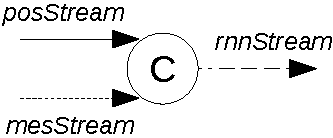
\includegraphics[scale=0.6]{img/dgm/SingleCache.pdf} 
}
\subfigure[A system with several caches]{
\label{subfig:rootRtree}
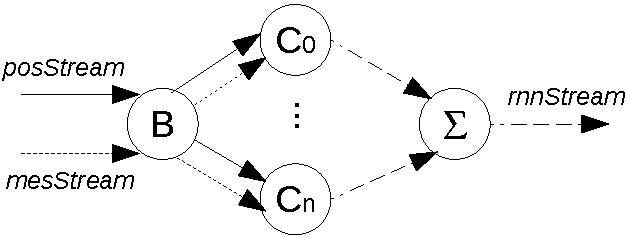
\includegraphics[scale=0.6]{img/dgm/MultiCache.pdf} 
}
\subfigure[A distributed R*-tree]{
\label{subfig:distributedRtree}
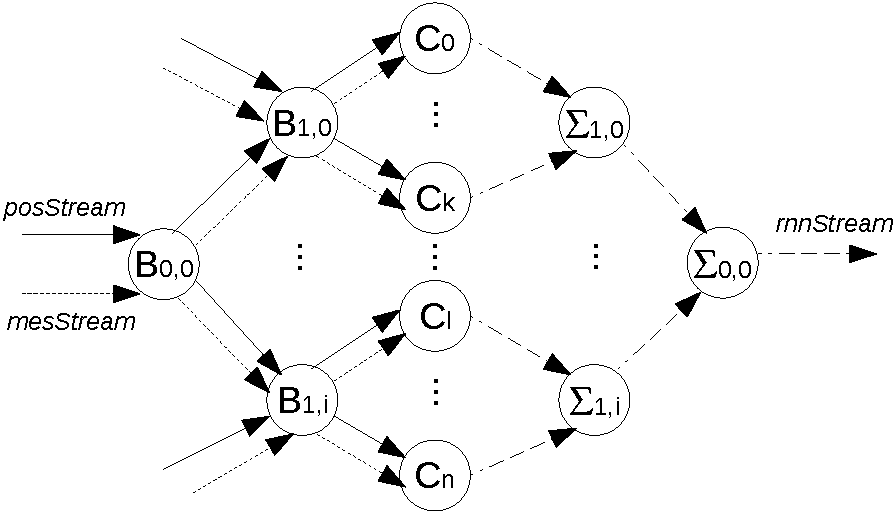
\includegraphics[scale=0.6]{img/dgm/DistributedTree.pdf} 
}
\caption{Distributing a geo-matching system}\label{fig:DistributedRtree}
\end{figure}

The problem of the system shown in figure \ref{subfig:localRtree} is that its processing capabilities are quite limited. Therefore, a distributed approach is required which spreads the load on several computers. Figure \ref{subfig:rootRtree} shows such a system. It consists of several caches $C_0$ to $C_n$ each of them owning an own R*-tree for caching current vehicle positions and responding to queries.

Furthermore, this system consists of balancer component $B$. It receives the incoming streams of vehicle positions and messages and decides to which of the different caches each single datum is sent. Similar to the root of an R*-tree, it keeps track of the MBRs of the different caches. A new vehicle position is basically sent to the cache with the nearest MBR. If $B$ receives a new message, it is only forwarded to the caches whose MBR intersects with the queried range. In the best case this is only one cache. But it could be several caches as well. Thus a special combiner component ($\Sigma$) is required which receives the nearest vehicle of each cache involved inte the query processing and returns the overall nearest neighbour.

A further responsibility of $B$ is the load balancing, i.e., the number of cached vehicle positions and queries in progress should be similar for all caches. Therefore, $B$ counts the number of vehicle positions and messages forwarded to the different caches. The load balancing is done by distributing the received vehicle positions according to special target ranges for the different caches. In the case of a balances system, these regions are equal to the MBRs. But if the load of a cache $C_i$ exceeds the load of a cache $C_j$ with a neighboured MBR, than the target range of $C_i$ is reduced and the range of $C_j$ increased. During the progress of the sliding window the MBRs of the caches will approach their target ranges.

In regular intervals, $B$ sends special requests to all caches to send the information about their current loads and MBRs back (not shown in figure \ref{subfig:rootRtree}). If $B$ receives the responses of all caches, it updates its calculated values. These update requests are performed asynchronously, i.e., the distribution of the incoming data is not blocked. This leads to a situation that the information received by the caches are not up to date any more. Therefore, $B$ caches all forwarding decisions from the time the updated request is sent until all caches have responded. Then these decisions are applied on the received load information and MBRs.

The disadvantage of this system is, that the single balancer component $B$ and combiner component $\Sigma$ can become bottlenecks. A future solution could be found when thinking of $B$ as the root of distributed R*-tree whose children are the trees stored in the different caches. If it is close to its processing limits, it creates child balancer components which are responsible for subregions of the overall MBR. Each of the children gets an input stream for all the data of its MBR. Data for regions which are not covered by the children are still received by the root. Whenever a balancer component is split the combiner components are split analogously. Such a system is illustrated in figure \ref{subfig:distributedRtree}.

\subsection{Experiment}\label{sec:experiment}


\section{Geographic Topic Analysis}
%--------------------------------------------------------------------
%\chapter{Topic Models}
%--------------------------------------------------------------------

The BuitenBeter dataset consists of 13,811 geo-tagged issues reported to the
office of public order in the Netherlands between July and September 2012.  Each
issue is assigned to one of 16 categories such as "poor road conditions", "Dirt
on the street" or "Graffiti".

Geographical co-occurrences of arbitrary categorical observations - such as
public order issues of the BuitenBeter dataset - can be used to discover latent
underlying factors that explain observations which co-occur more frequently than
expected by chance.  One method for detecting these latent factors is
probabilistic topic modelling, where grouped observations are modelled as being
sampled from mixtures of latent topics, which are probability distributions over
the set of distinct observations.

For the BuitenBeter dataset, we e.g. might expect that areas where graffities
are reported will see many reports of the category "Dirt on the street" since
both categories are related to urban environments. We model those environments
as hidden "topics".
  
Existing approaches for geographical topic modelling adopt topic models such as
latent Dirichlet allocation \cite{Blei:2003:LDA:944919.944937} and extend the
models by assigning distributions over locations to topics, or by introducing
latent geographical regions. In models which extend topics for spatial
distributions (such as two-dimensional normal distributions)
\cite{conf/wsdm/Sizov10}, topics with a complex (i.e. non-Gaussian) spatial
distribution cannot be detected. In models with latent, Gaussian distributed
regions \cite{conf/www/YinCHZH11}, documents within a complex shaped topic area
do not influence the topic distribution of distant documents within the same
area. Therefore, topics with a complex spatial distribution such as topics
distributed along coastlines, rivers or country borders are harder to detect by
such methods.  More elaborate models introduce artificial assumptions about the
structure of geographical distributions, e.g. by introducing hierarchical
structures \cite{ahmed13} in advance.
%Additionally, some approaches \cite{conf/www/MeiLSZ06,conf/www/YinCHZH11} do not model document-specific
%topic distributions. 

We introduce a novel geographical topic model which captures dependencies
between geographical regions to support the detection of topics with complex,
e.g. non-Gaus\-sian distributed spatial structures \cite{CCK1}.
%The model is based on a hierarchical Dirichlet process
%extended to support multiple base distributions, which we name MDP. 
%Our method thus is called the MDP-based geographical topic model (MGTM). 
%We use the MDP to dynamically smooth topic distributions between groups of spatially
%adjacent documents.

Our model differs from existing approaches in several aspects:

We model locations and words separately, as the separation of spatial clusters
and document semantics allows us to define meaningful neighbour relations
between spatially adjacent clusters. Our topic model takes a set of geographical
clusters as input.

We also expect that geographical clusters adjacent in space exhibit similar
topic distributions: Most geographical topics cannot be approximated by a simple
spatial probability distribution such as a Gaussian distribution and for these
complex topic areas, coherent sets of multiple spatial distributions are a
reasonable approximation.  Therefore we detect and smooth the topic distribution
of these adjacent regions to increase the probability of detecting coherent
topic areas.

The detection of geographical clusters is straight-forward: We use a mixture of
a fixed number of Fisher distributions -- distributions on a three dimensional
unit sphere similar to isotropic Gaussian distributions on a plane. The
parameters are fit using the approximation given by Banerjee et
al.~\cite{DBLP:journals/jmlr/BanerjeeDGS05} in an expectation-maximisation
algorithm.  In our model, each cluster is associated with a distribution over
the set of topics, sampled from a Dirichlet process (DP) with a common base
measure which is itself drawn from a DP with Dirichlet distributed multinomial
distributions over the set of categories as base measure.  For the smoothing of
topic distributions of adjacent clusters, we first define the adjacency relation
using the Delaunay triangulation \cite{journals/csur/Aurenhammer91} of the
cluster centroids.  Each public order issue report draws an own topic
distribution from a DP with a weighted mixture of the topic distribution of its
own geographical cluster and its neighbour clusters as base measure.  Finally,
each observed report category is drawn from its document-specific topic
distribution.  For a detailed description of the model and its parameters, we
refer to our paper \cite{CCK1}.

To train our model on the BuitenBeter dataset, we use 300 clusters and the
initial settings for the parameters $\beta = 0.5$, $\gamma = 1.0$, $\alpha_0 =
1.0$, $A = 99999$, $\delta = 1.0$. By setting $A$ to such a high value, we give
up document-specific topic distributions and sample the categories directly from
a mixture of region-specific topic distributions. All other parameters are set
to the values used in the paper \cite{CCK1}, except for the hyperparameters for
$A$, which is fixed.

For creating a comprehensible report, the detected topics can be characterised
by their most-likely categories:

Topic 1: \textit{Dirt on the street}, \ \textit{Other}, \ \textit{Graffities\\}
Topic 2: \textit{Damaged street light}, \ \textit{Bad road}\\
Topic 3: \textit{Obstacle by trees}, \ \textit{Weed}, \ \textit{Loose paving stones}, \ \textit{Bad road}, \ \textit{Idea/wish}\\
Topic 4: \textit{Other}, \ \textit{Weed}, \ \textit{Loose paving stones}, \ \textit{Bad road}, \ \textit{Damaged street light}, \ \textit{Idea/wish}


%for reduzing the size, set the width to 0.22\textwid
\begin{figure}[]
\centering
\subfigure[Topic 1]{
  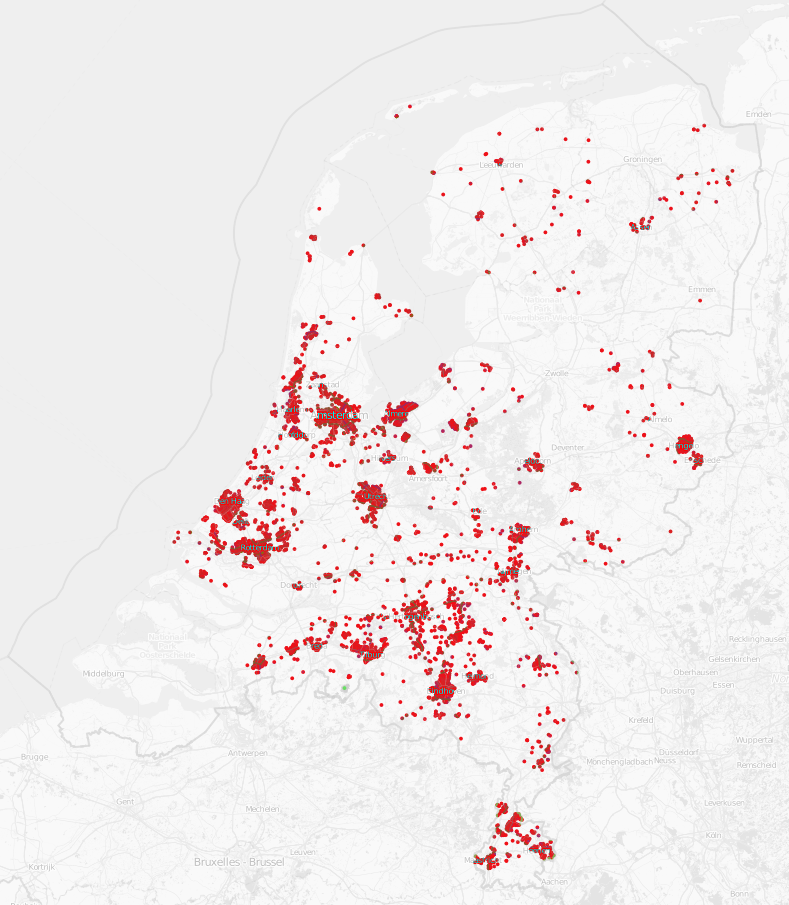
\includegraphics[width=0.3\textwidth,natwidth=556.19,natheight=432]{img/map/1.png}
  \label{plot:act20}
  \setcounter{subfigure}{1}
} 
\subfigure[Topic 2]{
  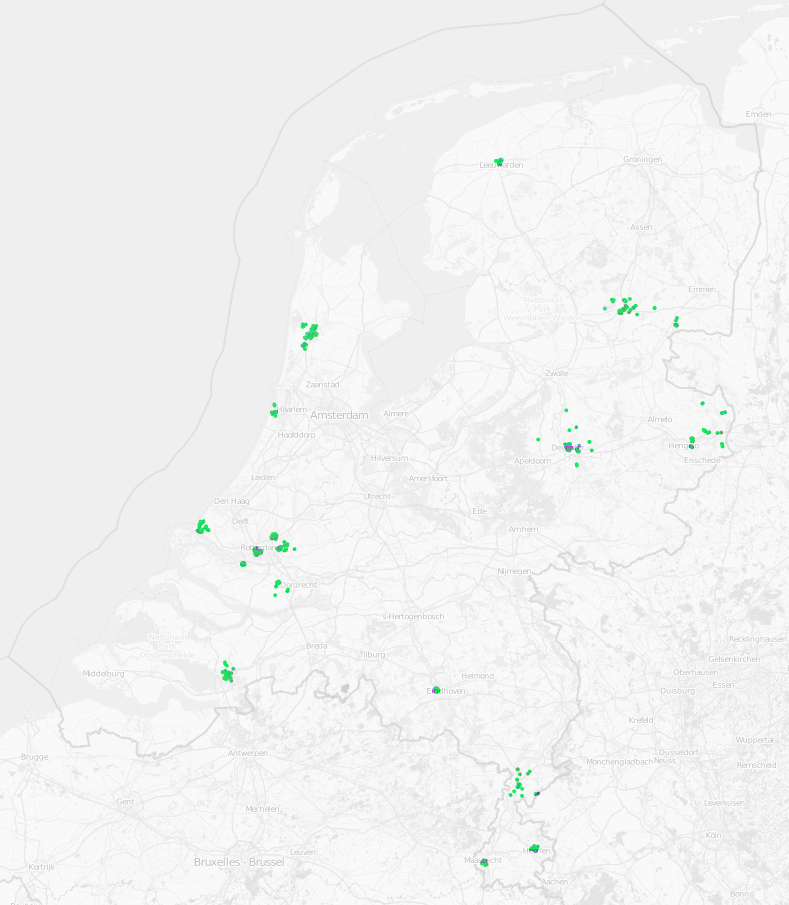
\includegraphics[width=0.3\textwidth,natwidth=556.19,natheight=432]{img/map/2.png}
  \label{plot:act20}
  \setcounter{subfigure}{2}
}

\subfigure[Topic 3]{
  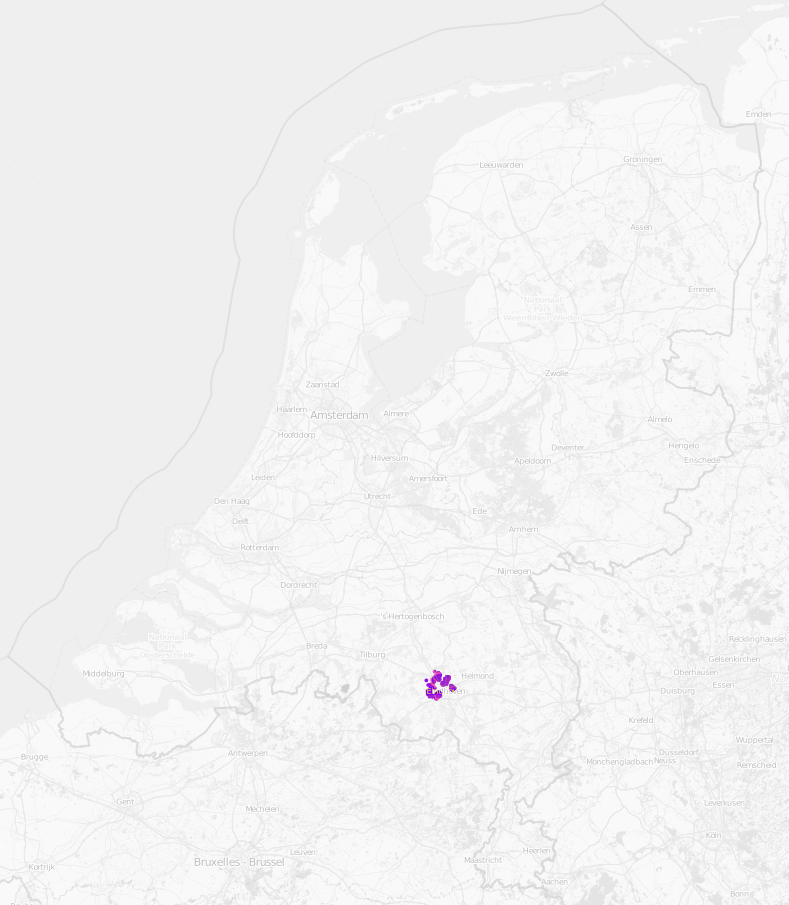
\includegraphics[width=0.3\textwidth,natwidth=556.19,natheight=432]{img/map/3.png}
  \label{plot:act20}
  \setcounter{subfigure}{3}
}
\subfigure[Topic 4]{
  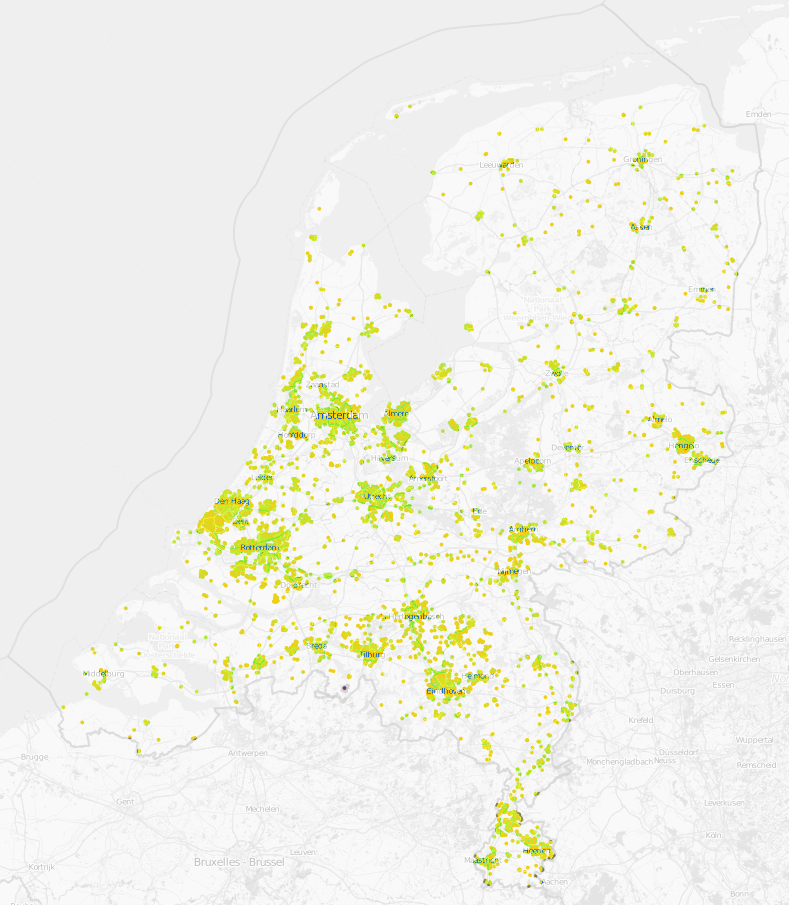
\includegraphics[width=0.3\textwidth,natwidth=556.19,natheight=432]{img/map/4.png}
  \label{plot:act20}
  \setcounter{subfigure}{4}
} 

\caption{
  Document positions of reports with above-average probabilities for Topic 1-4 on the map of the Netherlands.
}
\label{fig:netmaps}
\end{figure}

The position of documents with an above-average probability for each topic are
shown in \vbox{Figure \ref{fig:netmaps}}.  We see that, as expected, Topic 1 is
only observed in the area of larger cities, whilst Topic 4 is present across the
whole country.  Topic 2 occurs mostly within city centres.  Topic 3 is observed
in the area of Eindhoven for which different categories were available in the
BuitenBeter application.

%%% Local Variables: 
%%% mode: latex
%%% TeX-master: "../D1-2"
%%% End: 


\bibliography{D1-2}

\end{document}
